\newpage
\section{Preprocessing}
We approach preprocessing in two steps. In the first step we clean the data set\todo{data set vereinheitlichen} based on knowledge we obtained in the Data Understanding section and further analysis. 
Secondly, we transform the data using hyperparameter tuning.
%Secondly, we try many different approaches to transform the data, in instances where we can not be certain about the best method. \todo{der letzte halbsatz passt nicht}

\subsection{Cleaning}
Firstly, we implement a custom loading function to transform the 4 datasets into a csv format, so we can use it further on.

We remove the false predictors lmt, ladprox, laddist, diag, cxmain, ramus, om1, om2, rcaprox and rcadist, as our target variable num is a combination of these according to the UCI. %Nochmal angucken mit Finn.

Furthermore, the features thalsev, thalpul, lvx1, lvx2, lvx3, lvx4, lvf, dummy\todo{dummy ist nicht beschrieben} and junk are considered irrelevant by the UCI, so we also drop them. Other irrelevant attributes we remove are IDs(id,ccf), constants \todo{or empty features}(name, earlobe, restckm, exerckm) and dates of medical examinations (ekgmo, ekgday, ekgyr, cmo, cday, cyr). We consider these dates irrelevant because we assume that the date of  an examination does not affect its outcome. 

We drop the feature pncaden because it is the sum of painlox, painexer and relrest and therefore contains no additional information. 

The features cp, restecg, slope, ca and restwm were oneHotEncoded as they represent categorical values.

When checking for inconsistencies between features, we detected that thaltime is sometimes lower than thaldur\todo{ausschreiben, was die feature bedeuten, dass fehlt allgemein bis zu diesem Zeitpunkt} . As thaltime describes the moment \todo{fachbegriffe erklären bzw verweise rein} a measurement is taken within the exercise, it has to be lower than the duration of the exercise thaldur. We replace thaltime by \texttt{NaN} in all 17 instances that do not satisfy this criterion. 

Also, the maximum heart rate (thalach) was replaced with \texttt{NaN} if it was lower than the heart rate at rest (thalrest).

\begin{figure}[h]
	\centering
	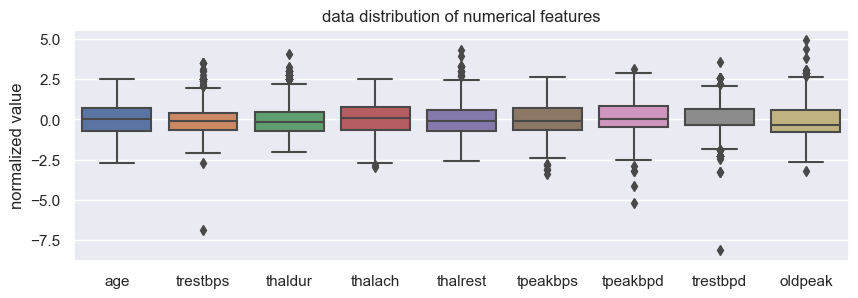
\includegraphics[width=0.7\textwidth]{images/dataDistribution.png}
	\caption{data distribution of all numeric elements}
	\label{fig:dataDistribution}
\end{figure}
As shown in \ref{fig:dataDistribution} we created a normalized box plot of all numeric features to check for outliers. The features trestbps and trestbpd show extreme outliers with a value of 0. These are incorrectly\todo{assumed?} specified \texttt{NaN}s and are therefore replaced by \texttt{NaN}. All other outliers are not as extreme and come in groups. As the data contains sick persons, values diverging from the norm are expected. For these reasons we decided to keep these outliers as they can be a strong indication of a heart disease.

The remaining features were analysed regarding their pearson correlation. Only two pairs of features with substantive amount of data (less than 75\% \texttt{NaN}s) have a very strong correlation (\>80\%).  

These are cp\_4$\leftrightarrow$painexer and rldv5$\leftrightarrow$rldv5e. The highest correlation is between cp\_4 and painexer. The feature cp\_4, which was oneHotEncoded from the categorical variable cp, describes whether the patient has no chest pain at rest. Painexer describes whether the patient only has pain when exercising. 

Concluding from the high correlation between the EKG amplitude when resting (rldv5) and the EKG amplitude when exercising (rldv5e), we decided to create a new feature(rldv5\_diff) by using the difference between these. We did the same with resting heart rate and maximum heart rate (thal\_diff = thalach - thalrest). 

Furthermore, we enrich the feature smoke using years and cigs. Hereby, we reduce the number of \texttt{NaN}s from 74\% to 43\%. 

\subsection{Hyperparameter Tuning }
Additionally to the hyperparamter tuning of the estimators, which is described in LINK\_CHAPTER\_3, we also optimize which method is used with which hyperparameters in the preprocessing steps.
%For hyperparameters and methods where we could not be certain, we try out multiple different combinations.\todo{liest sich doof}

Firstly, we try binning the feature age. We choose either 2 or 5 bins or no binning at all. We decided to use equal width binning so that the age groups are simpler and more intuitive to a doctor.

\begin{figure}[h]
	\centering
	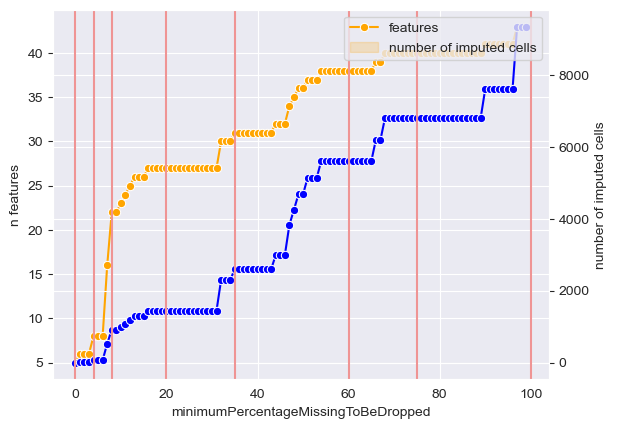
\includegraphics[width=0.7\textwidth]{images/percentageToBeDropped.png}
	\caption{Number of features and values to be imputed by number of \texttt{NaN}s}
	\label{fig:percentageToBeDropped}
\end{figure}
Figure \ref{fig:percentageToBeDropped} shows the number of features, that have less than a certain number of missing data and how many cells we would need to impute if we included these features. It becomes apparent that there are certain steps where the number of features goes up a lot. To decide when a feature is included based on the number of missing values, we try the steps 0, 4, 8, 20, 35, 60, 75 and 100 \% in the model. They are shown as vertical lines in the graph. Additionally, we decided to drop features based on their correlation. For this we decided to use the steps [X,X,X,X].

To impute the missing data we use a simple imputer. Missing values are replaced by the mean, median or mode of the feature. We decided against using a KNN imputer, because it is computationally much more expensive. The iterative imputer is not used, as it is still experimental and therefore subject to change.

To account for the different ranges of the features different scalers are tried out. We only use scalers that are applicable for all floats as some features contain negative values.
We compare the MaxAbsScaler, MinMaxScaler, PowerTransformer, RobustScaler, Standardscaler and Normalizer. As the hyperparameters of most scalers turn on or off core functionalities of the scaler, we decided to only tune the hyperparameter norm of the Normalizer with the norms l1, l2 and max.

To account for the different amounts of healthy and unhealthy patients we try oversampling and undersampling in the training data in comparison to passing the values through.


%The \textbf{MaxAbsScaler} scales the values of each feature by the maximum absolute value. Therefore, all values in [-1,1] can occur after scaling. \newline
%Using the \textbf{MinMaxScaler} results in values in [0,1] by shifting by the negative minimum and scaling by $maximum - minimum$\newline
%The values were normalized using the norms l1,l2 and max in the \textbf{Normalizer}. \newline
%The \textbf{PowerTransformer} alters the data to represent a gaußian like distribution. This is mostly used if heteroskedasticity occurs in the data. It was tried to fit the data to a standard normal distribution and without shifting and scaling by its mean and variance. \newline
%The \textbf{RobustScaler} was tried with and without scaling by the interquartile range and with and without shifting beforehand.\newline
%The \textbf{Standardscaler} was used with and without shifting by the mean and scaling by the standard deviation.\newline
%It was also tried, manly for comparison, to \textbf{passthrough} the values as they are.\newline